% A simple template for LaTeX documents
% 
% To produce pdf run:
%   $ pdflatex paper.tex 
%


\documentclass[12pt]{article}

% Begin paragraphs with new line
\usepackage{parskip}  

% Change margin size
\usepackage[margin=1in]{geometry}   

% Graphics Example:  (PDF's make for good plots)
\usepackage{graphicx}               
% \centerline{\includegraphics{figure.pdf}}

% subfigures, side by side
\usepackage{subcaption}

% hyperlinks
\usepackage{hyperref}

% Blocks of code
\usepackage{listings}
\lstset{basicstyle=\ttfamily, title=\lstname}
% Insert code like this. replace `plot.R` with file name.
% \lstinputlisting{plot.R}

% Monospaced fonts
%\usepackage{inconsolata}
% GNU \texttt{make} is a nice tool.

% Supports proof environment
\usepackage{amsthm}

% Allows writing \implies and align*
\usepackage{amsmath}

% Allows mathbb{R}
\usepackage{amsfonts}

% Numbers in scientific notation
% \usepackage{siunitx}

% Use tables generated by pandas
\usepackage{booktabs}

% Allows umlaut and non ascii characters
\usepackage[utf8]{inputenc}

% norm and infinity norm
\newcommand{\norm}[1]{\left\lVert#1\right\rVert}
\newcommand{\inorm}[1]{\left\lVert#1\right\rVert_\infty}

% Statistics essentials
\newcommand{\iid}{\text{ iid }}
\newcommand{\Exp}{\operatorname{E}}
\newcommand{\Var}{\operatorname{Var}}
\newcommand{\Cov}{\operatorname{Cov}}


%%%%%%%%%%%%%%%%%%%%%%%%%%%%%%%%%%%%%%%%%%%%%%%%%%%%%%%%%%%%

\begin{document}

\title{Code Analysis Project Proposal}
\date{\today}
\author{Clark Fitzgerald}
\maketitle

\begin{abstract}

\end{abstract}

\section{Introduction}
%%%%%%%%%%%%%%%%%%%%%%%%%%%%%%%%%%%%%%%%%%%%%%%%%%%%%%%%%%%%

The idea behind code analysis is to treat the code itself as a data
structure. This is an old idea, the R language reference cites the Lisp
language as the inspiration.

The interpreter works in a simple way. The \texttt{Rscript} command will go
through a file line by line and parses then
evaluates each statement. R's \texttt{source()} function on the other hand
first parses the whole thing, and then evaluates it all. We propose to
first parse and then examine whole scripts at a time, from just a couple
lines to a few hundred lines of code.  The whole script is parsed into a
directed graph data structure. Nodes contain the expressions and the edges
contain the dependence information.  TODO: but what about control flow?
loops?

\section{Dependencies}
%%%%%%%%%%%%%%%%%%%%%%%%%%%%%%%%%%%%%%%%%%%%%%%%%%%%%%%%%%%%

We need to start out with some definitions and basic concepts to make all
of this precise. The following material is from the R
Language Reference \cite{Rlang}.

``A \textbf{statement} is a
syntactically correct collection of tokens.'' Less formally one can think of
a statement as a single line of code. The `line' rule doesn't always hold in practice,
since a semicolon can put two statements on one line, and a single
statement may span multiple lines.

\begin{verbatim}
# Two statements on line
a <- 1; b <- 2

# One statement on multiple lines
plot(lm(y ~ x,
        data = xydata))
\end{verbatim}

\textbf{symbol} is a variable name such as \textbf{a, b} above.  The words
symbol, variable, and name are used interchangeably. For consistency I'll
stick with symbol.

Assignment is the binding of a symbol to an R object. Complex assignment

``An \textbf{expression} contains one or more statements.'' Expression objects
in the langauge contain parsed but unevaluated statements. 

Statements can be grouped together using braces to form a \textbf{block}.
Since expressions can be nested, we can consider a block just a special
type of expression.

\begin{verbatim}
{
a <- 1
b <- 2
}
\end{verbatim}

TODO: Not sure how to handle blocks. One option is to go inside them and
look at all the individual statements. The other option, which seems easier
at first, is to do what CodeDepends does and group them into one
single logical unit. Presumably if a programmer writes a block like this
they intend the whole thing to execute together. One typically sees blocks
along with \texttt{if} statements.

But in the end I think I'll have to recurse inside the expressions at the
script level, but not down into the supporting library R code. For example, to
get a minimum set of code to perform a final operation one would need to go
into a block.

So how do we detect dependencies in code?

Idea talking with math students- count the incoming and outgoing edges. Use
this info.

\section{Graph Construction}

The graphs can be built sequentially, as the script is parsed.

The nodes in the graph are code expressions.
An expression may do any combination of the following things:
\begin{enumerate}
    \item Define new symbols
    \item Use existing symbols
    \item Redefine existing symbols
\end{enumerate}

Consider the following simple script:

\begin{verbatim}
x <- 1:10   # expression 1
plot(x)     # expression 2
x <- 1:5    # expression 3
plot(x)     # expression 4
\end{verbatim}

The first expression defines the new symbol \texttt{x}. The third
expression redefines \texttt{x} without making use of the existing
definition.

The second expression uses \texttt{x}, so we define an edge from node 1 to 2.
More generally we define an edge from the most recent expression that
updated \texttt{x}. Therefore the fourth expression creates an edge from 3
to 4.

The complete graph is then:

\begin{verbatim}
1 -> 2
3 -> 4
\end{verbatim}

But how will we know if the symbol exists? After parsing we could
potentially see the timelines recording which symbols live, and if they are
ever removed. This may depend on conditional statements, which we can't
know. The safe thing then seems to just assume that they will be used.

TODO: Is this just for the global namespace? How will it be different for
others? I think it's ok to just focus on the globals first. Environments in
general may require more thought.

``R adheres to a set of rules that are called lexical scope. This means the
variable bindings in effect at the time the expression was created are used
to provide values for any unbound symbols in the expression.''
\cite{Rlang} A primary goal is to respect R's lexical scoping rules.


\section{Code graph and parse tree }
%%%%%%%%%%%%%%%%%%%%%%%%%%%%%%%%%%%%%%%%%%%%%%%%%%%%%%%%%%%%

The code graph and related data structures are related to the parsed
script, which we'll refer to as the \textbf{parse tree}. Since the parser
doesn't care about white space different scripts can produce the same parse
tree. R's \texttt{getParseData()} preserves all of the source
information, and this can be very helpful for debugging or IDE's. Later
this might be useful for injecting code.
For our immediate purposes scripts differing only in comments and white space can be
considered the same, which gives a 1 to 1 relationship between scripts and
parse trees. 

Many parse trees can give rise to the same code graph. For
example, the code graph shouldn't care if one uses \texttt{<-} or
\texttt{=} for assignment. Nor will it care about the ordering of two
adjacent lines binding a symbol to a literal constant:

\begin{verbatim}
a <- 1
b <- 2
\end{verbatim}

Therefore we lose information by converting from a parse tree to this code
graph.

\lstinputlisting[language=R, caption=Simple script, label=list:ab]{../experiments/ast/ab.R}

\begin{figure}
\centering
\begin{subfigure}{.6\textwidth}
    \centering
    \includegraphics[width=.8\linewidth]{../experiments/ast/ast.pdf}
    \caption{Parse tree}
    \label{fig:ast}
\end{subfigure}%
\begin{subfigure}{.4\textwidth}
  \centering
  \includegraphics[width=.8\linewidth]{../experiments/ast/codegraph.pdf}
  \caption{Expression dependency graph}
  \label{fig:codegraph}
\end{subfigure}
\caption{Different representations of the script in Listing \ref{list:ab}}
%\label{fig:test}
\end{figure}

For visualizing the control flow and dependencies it's important to have the entire
expression available in the node as in Figure \ref{fig:codegraph}. This
lets users easily connect the graph with the source file. Another thought
that would make this easier- put the source code line number along with the
line of code.


\section{How CodeDepends works}
%%%%%%%%%%%%%%%%%%%%%%%%%%%%%%%%%%%%%%%%%%%%%%%%%%%%%%%%%%%%

The parsing uses an object oriented wrapper around R's builtin \texttt{parse()}
which handles different file types and other arguments.

The workhorse function looks to be \texttt{getInputs.language()}. This
takes in an expression. It recurses through expressions until it finds
calls, functions, or ???.
For functions it uses
\texttt{codetools::findGlobals()} to record global usage and function
calls.
For the rest it uses a collector object to move through the code and
collect information about variable names, side effects, and functions
called. There are many special cases handled in functionHandlers.R, such as
\texttt{\$, rm, for} and non standard evaluation. Seems quite complicated.
Comments mention dplyr operations.

How much of this complexity can be handled by something like
\texttt{getParseData()}? This provides a nice data frame. I think that I
need to graph this to see how well I understand it.

From what I see here CodeDepends uses the tokens
somewhat indirectly, through functions like \texttt{is.name()}. 
How long would it take to refactor CodeDepends so that I understand it?



\section{Related Work}
%%%%%%%%%%%%%%%%%%%%%%%%%%%%%%%%%%%%%%%%%%%%%%%%%%%%%%%%%%%%

Jim Hester's covr package \cite{R-covr} checks unit test coverage of R
code. It is a practical example of computing on the language,
programmatically modifying the code by recording calls as they are made.

TODO Gives me an idea... a similar strategy might work to collect timings and
resource usage for functions called with various data sizes. Then we can
use this info to programmatically modify the code: ie. if $n > 1000$ then
run a multicore version. This is something like Profile Guided Optimization
(PGO). This technique is now being used for Python. Could R use it too?

\section{Applications}
%%%%%%%%%%%%%%%%%%%%%%%%%%%%%%%%%%%%%%%%%%%%%%%%%%%%%%%%%%%%


What are all the useful things to do when rewriting code?  Duncan's very
helpful docs here http://www.omegahat.net/CodeDepends/design.pdf give a
handful of reasons.

Other things that I can think of:

Identification and elimination of dead code.

- Given a big ugly script, pull out the minimal set of code to produce a
  final result. For example, everything needed to make `plot(finalresult)`.
- Parse Rhistory to find the minimal set of code to reproduce a result.
- Separate single scripts into multiple scripts if they actually have two
  independent sequences of computation.

These ideas stay much closer to the syntax and language of R compared to
what Nick is doing.

\section{Detecting Parallelism}
%%%%%%%%%%%%%%%%%%%%%%%%%%%%%%%%%%%%%%%%%%%%%%%%%%%%%%%%%%%%

Not sure how to generally detect where the possibilities for
parallel are. In a simple case of k obvious threads with one common
ancestor and common child there is an obvious option:

Remove the common ancestor and child and select the k disjoint subgraphs
between them.

Alternatively:

1. Start at the top of the graph, and move down until one node has
multiple children. Gather those child threads into 2 groups.
2. Same thing starting at the bottom.

The most straightforward thing to do right now is take a more complex
graph, say something like this:

\centerline{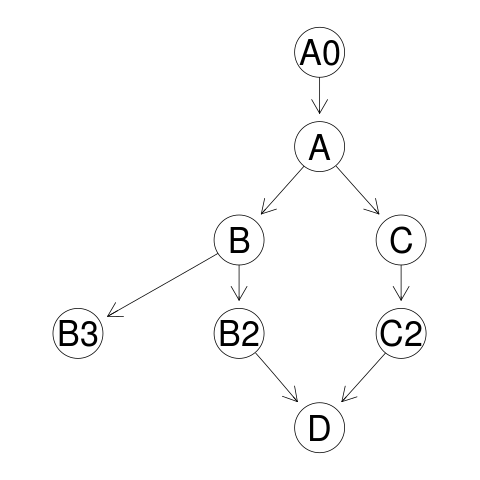
\includegraphics{../codedepends/larger_graph.png}}


And attempt to collapse the structure into one where the parallel threads
become obvious:

\centerline{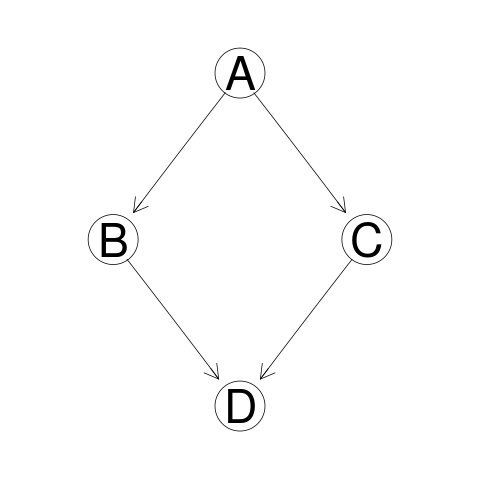
\includegraphics{../codedepends/simple_graph.png}}

The essential part for the multiprocessing is to have many "adjacent"
threads (is there a correct graph term for this?)
Optionally the adjacent threads can share a common parent and or child
nodes.

\section{The right data structure}
%%%%%%%%%%%%%%%%%%%%%%%%%%%%%%%%%%%%%%%%%%%%%%%%%%%%%%%%%%%%

If the intermediate variable `b` is not used anywhere we probably want to
collapse the following into a single block of code, since it has to happen
sequentially. Therefore adding `future` here can't help at all. Unless it
should happen at the same time as another block... then two blocks can
execute simulataneously.

\begin{verbatim}
# Begin block
a = 100
b = a + 5
c = sum(b)
# end block
\end{verbatim}

\section{Hard things}
%%%%%%%%%%%%%%%%%%%%%%%%%%%%%%%%%%%%%%%%%%%%%%%%%%%%%%%%%%%%

`fit = lm(y ~ x)` doesn't detect the dependency of `fit` on `x, y`.

Following the control flow for `lm` we see the following calls:
`model.matrix.lm`, `model.frame.default`, `as.formula`. But eventually this
`y ~ x` itself must be evaluated in which case `.Primitive("~")` is called,
which certainly does something weird. But what?

Haven't yet checked things like:
`<<-, assign`

Recursion? Iterating updates?

\newpage

\bibliographystyle{plain}
\bibliography{citations} 

\end{document}
